\chapter{Via Purifico}

\begin{enumerate}
    \item Run up past the first telepad
    \item Go to the second telepad and travel north.
\end{enumerate}
\bothvfill
\winvfill
\begin{spheregrid}
    \begin{itemize}
        \auronf
        \begin{itemize}
            \item Move $\rightarrow\rightarrow\rightarrow$
            \item Level 2 Keysphere
            \item Move $\rightarrow x4$ (or Hold $\rightarrow$)
            \item Level 2 Keysphere
            \item Move $\uparrow\uparrow$ ($\uparrow\leftarrow$ if you are not on the correct Node)
            \item Mag+3
        \end{itemize}
        \ifthenelse{\equal{\colstyle}{multi}}{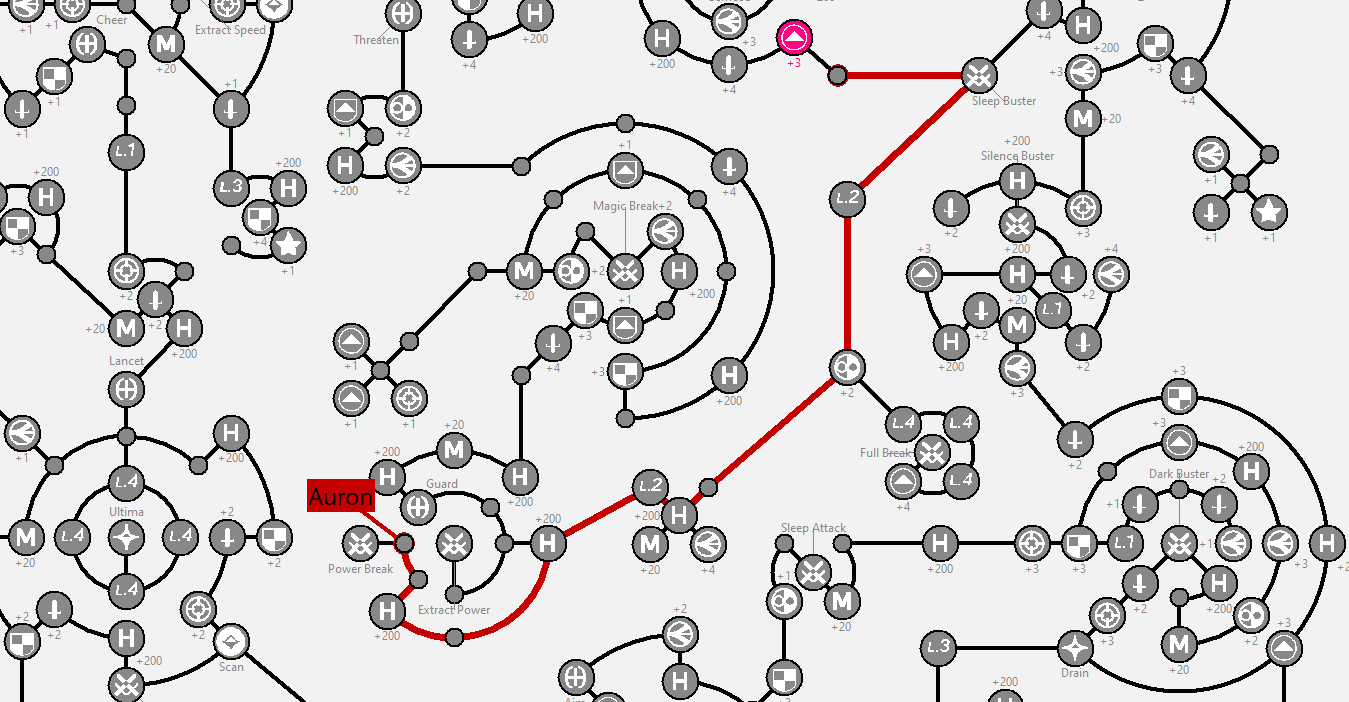
\includegraphics[width=.8\columnwidth]{graphics/Auron_Via_Purifico}}{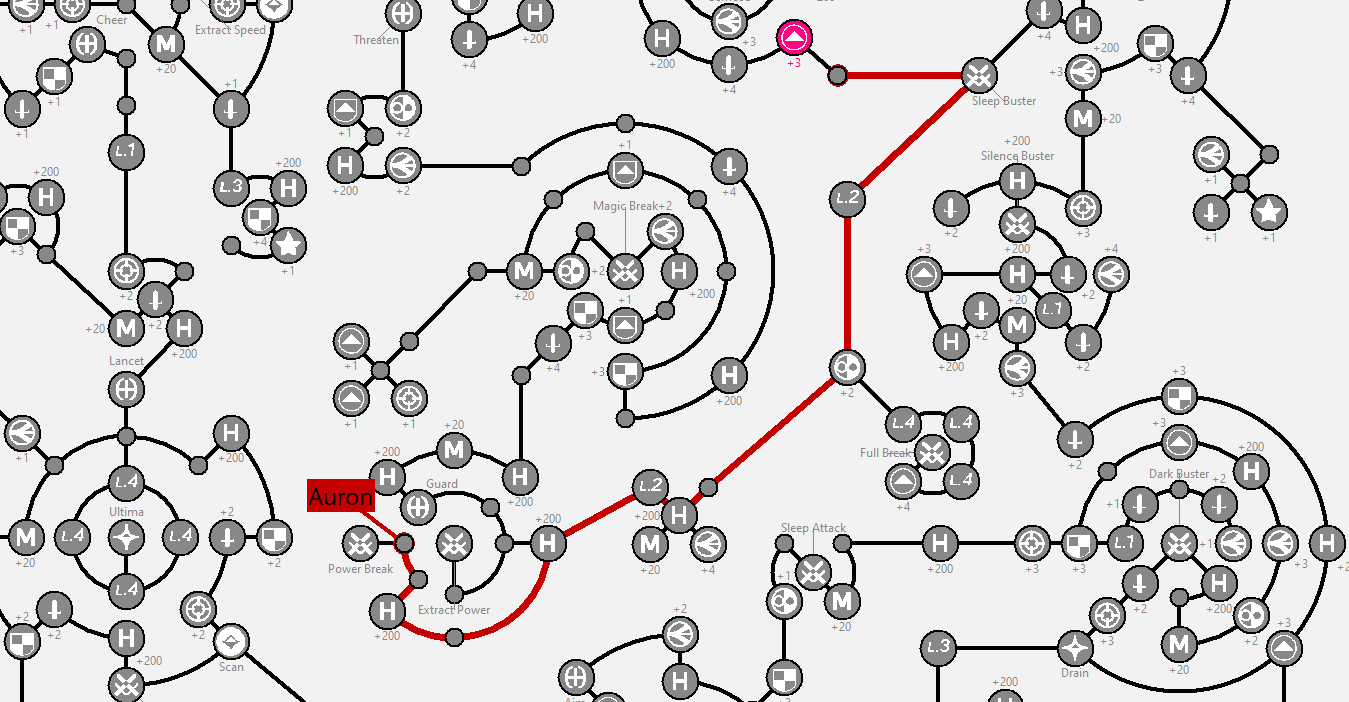
\includegraphics[width=.45\columnwidth]{graphics/Auron_Via_Purifico}}
        \yunaf
        \begin{itemize}
            \begin{multicols}{2}
                \item Move $\uparrow\uparrow$
                \item Level 4 Keysphere
                \item Move $\rightarrow x3 \uparrow$
                \item Str+2, Str+2, Str+2
                \item Teleport Sphere to \auron's Magic Node $\uparrow$
                \item Use Magic Sphere
                \item Str+4, Mag+3, Mag+4
                \item Move $\rightarrow\rightarrow\rightarrow\uparrow$
                \item Mag+3, HP+200, Str+4
                \item Move $\rightarrow$
                \item Def+3, Str+4
                \item Move $\leftarrow\downarrow$
                \item Agi+3, MP+20
                \item Move $\leftarrow\downarrow$
                \item HP+200, Str+2
                \item Move $\downarrow\downarrow$
                \item HP+200, Str+2, Mag+3
                \item Level 1 Keysphere
                \item Move $\searrow\searrow$
                \item Agi+4, Str+2
                \item Move $\leftarrow\leftarrow$
                \item Str+2
                \item Move $\downarrow$
                \item Str+2, MP+20, Agi+3
            \end{multicols}
        \end{itemize}
        \ifthenelse{\equal{\colstyle}{multi}}{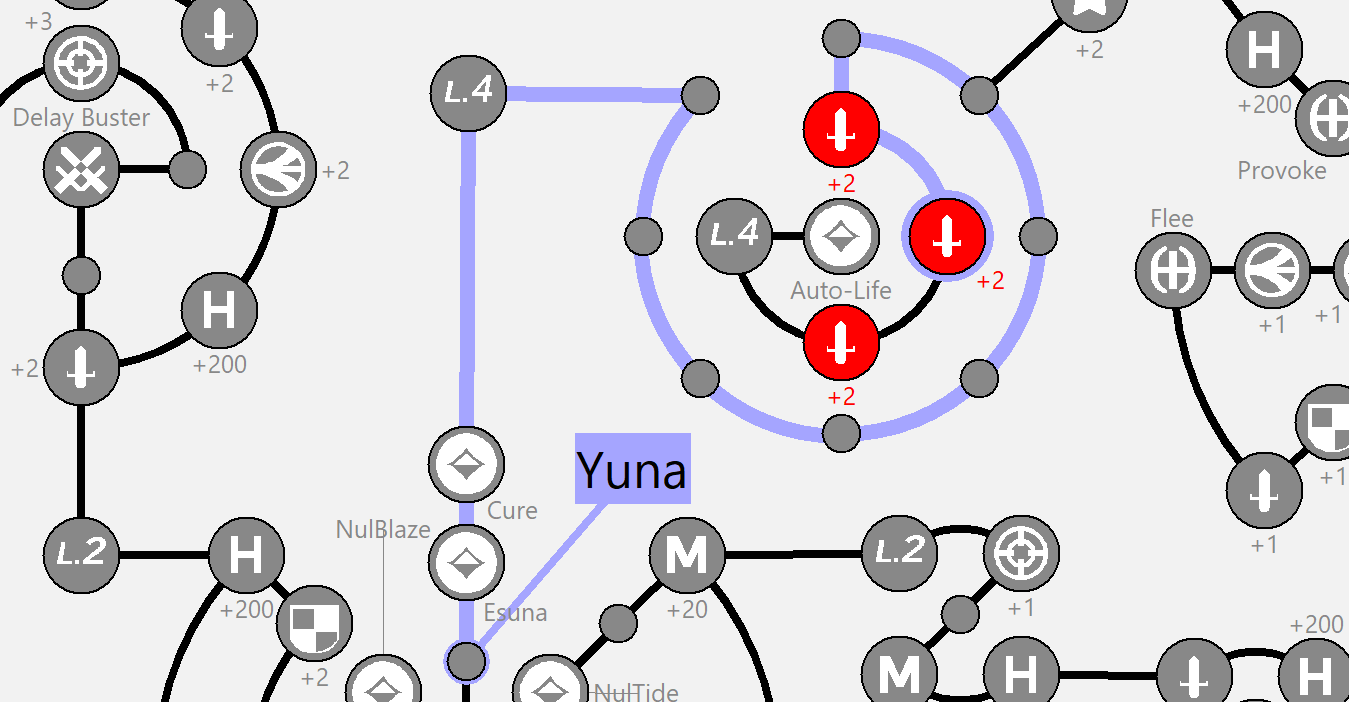
\includegraphics[width=.8\columnwidth]{graphics/via_purifico_yuna_1}}{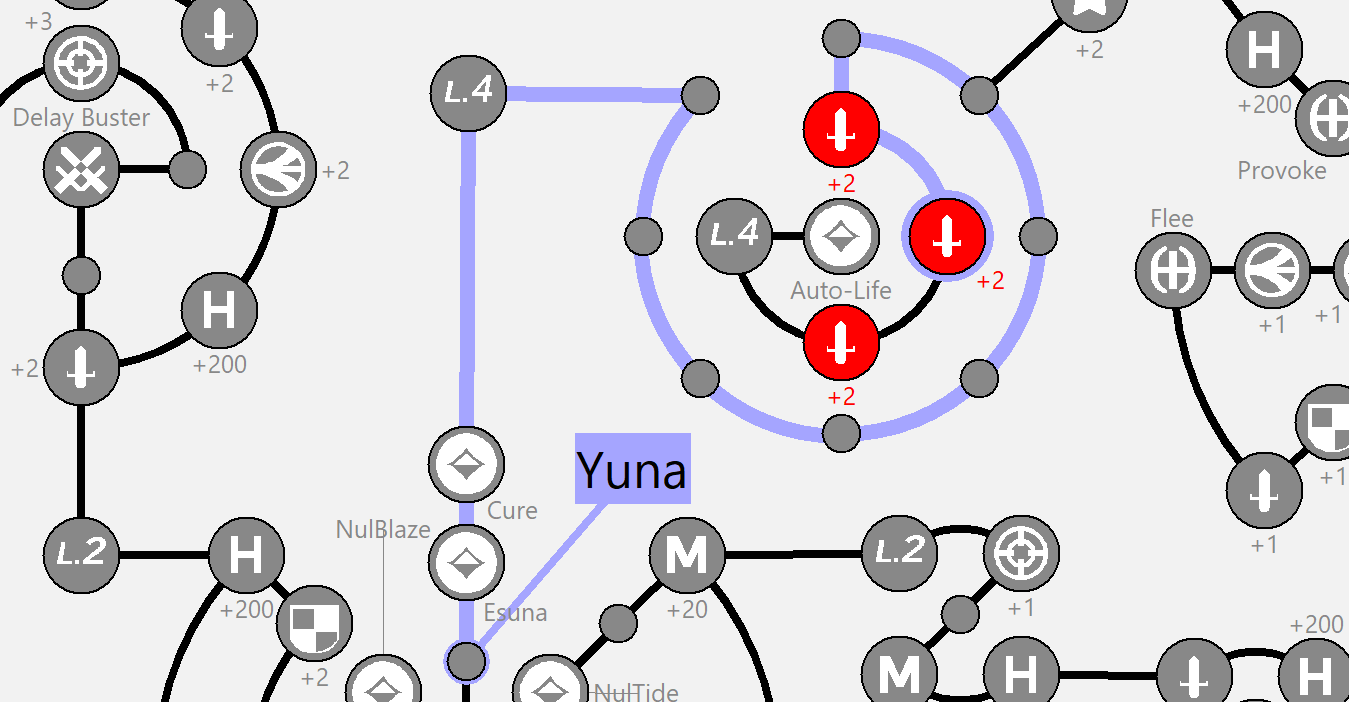
\includegraphics[width=.45\columnwidth]{graphics/via_purifico_yuna_1}}
        \ifthenelse{\equal{\colstyle}{multi}}{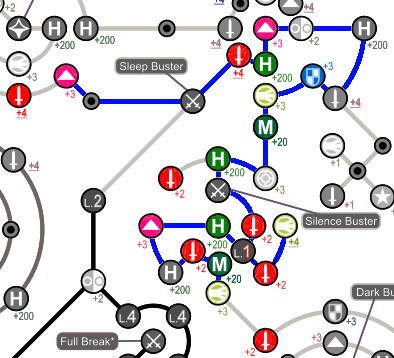
\includegraphics[width=.8\columnwidth]{graphics/via_purifico_yuna_2}}{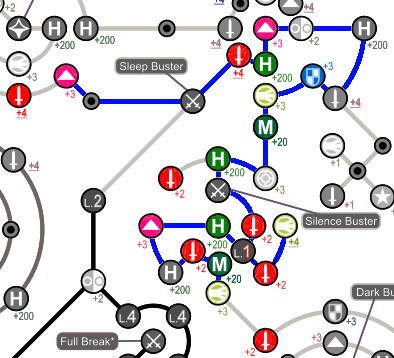
\includegraphics[width=.45\columnwidth]{graphics/via_purifico_yuna_2}}
    \end{itemize}
\end{spheregrid}
\begin{enumerate}[resume]
    \item You need 13 Power Spheres and 7 Speed Spheres for the rest of the run.
    \item \save
    \item Keep track of how many things you kill here.
\end{enumerate}
\begin{encounters}
    \begin{itemize}
        \item Maze Larva: Summon \ixion, Attack
    \end{itemize}
\end{encounters}
\bothvfill
\winvfill
\lossvfill
\begin{battle}{Isaaru}
    \begin{itemize}
        \item Grothia (8000 HP):
        \begin{itemize}
            \summon{\bahamut}
            \bahamutf Attack
        \end{itemize}
        \item Pterya (12000 HP):
        \begin{itemize}
            \summon{\bahamut}
            \bahamutf Attack
        \end{itemize}
        \item Spathi (20000 HP):
        \begin{itemize}
            \summon{\ixion}
            \ixionf Attack x4
        \end{itemize}
    \end{itemize}
\end{battle}
\begin{enumerate}[resume]
    \item You can use the underwater chest on the right at the start to buy a Speed Distiller (this is the last convenient opportunity to acquire Speed Spheres) or a Power Distiller.
    \item If needed, you can attack a Phlegias or a Sahagin with \tidus\ for 2x Power Spheres (only do so on a non-Ambush).
    \item Swim up, then up again when the camera changes. 
\end{enumerate}
\begin{battle}{Evrae Altana}
    \begin{itemize}
        \item Anyone: 1 Power/Speed Distiller if needed
        \item Anyone: Elixir/Phoenix Down x2 Evrae Altana
    \end{itemize}
\end{battle}
\begin{enumerate}[resume]
    \item Swim to exit, \sd
\end{enumerate}
\ 
\bothvfill
\ \bothnewline
\bothcb
\ 

\bothnpsingle